\documentclass[a4paper, oneside, 11pt]{report}
\usepackage{epsfig,pifont,float,multirow,amsmath,amssymb,url}
\newcommand{\mc}{\multicolumn{1}{c|}}
\newcommand{\mb}{\mathbf}
\newcommand{\mi}{\mathit}
\newcommand{\oa}{\overrightarrow}
\newcommand{\bs}{\boldsymbol}
\newcommand{\ra}{\rightarrow}
\newcommand{\la}{\leftarrow}
\usepackage{algorithm}
\usepackage{algorithmic}
\topmargin = 0pt
\voffset = -80pt
\oddsidemargin = 15pt
\textwidth = 425pt
\textheight = 750pt
\usepackage[parfill]{parskip}
\usepackage{blindtext}

\begin{document}

\begin{titlepage}
\begin{center}
\rule{12cm}{1mm} \\
\vspace{1cm}
{\large  CMP-7014B Computer Games Laboratory}
\vspace{7.5cm}
\\{\Large Project Report - May 2019}
\vspace{1.5cm}
\\{\LARGE DunCraw: The Third Realm}
\vspace{1.0cm}
\\{\Large Group members: \\ Ben Longhurst, Ryan Phelan and Sam Griffiths}
\vspace{10.0cm}
\\{\large School of Computing Sciences, University of East Anglia}
\\ \rule{12cm}{0.5mm}
\\ \hspace{8.5cm} {\large Version 1.0}
\end{center}
\end{titlepage}
\tableofcontents

\setcounter{page}{1}
%\pagenumbering{roman}
%\newpage

\chapter{Introduction}
DunCraw: The Third Realm is a 3D fantasy dungeon crawler which features a variety of graphical and algorithmic techniques such as advanced lighting, artificial intelligence and procedural content generation. The objective of the game is to escape the mysterious realm by acquiring six keys found deep within the dungeon. Venturing through the dungeon portal comes with great risk however, as the player must battle the fireball-throwing minotaurs which guard an ancient maze.

The game is programmed using OpenGL~\cite{opengl} with C++, adhering to the Entity-Component-System (ECS) design pattern (Section~\ref{section-ecs}) with the EnTT library~\cite{entt}. In following ECS, the game intends to simplify code architecture and therefore improve rendering efficiency. 

\section{Aim and Objectives}\label{section-requirements}
In terms of goals, the project aims to create a game which showcases graphical and algorithmic techniques implemented by the team. The game-play itself is not a focus, though it should feel ``complete'' in the sense that there is an objective, win and loss states. The following minimal product requirements were defined for the game:

\begin{itemize}
    \item The game must have a clear and objective ending
    \item The game must be verified completeable with no game-breaking bugs
    \item The current game state must be clear (current health, keys collected etc.)
    \item The game must have an enemy threat
    \item The framerate must remain stable
    \item The scene must be believable as a fantasy dungeon
    \item The scene lighting must be appear realistic
    \item The player must collide with walls, projectiles and game objects
\end{itemize}

\section{MoSCoW}
To better prioritise objectives, a MoSCoW analysis was produced (Figure~\ref{moscow-1}). The ``Must Have'' objectives were prioritised as components necessary to development of a simple scene, which could be considered a minimal submission. Those outlined in ``Should Have'' then aim to extend this scene with simplistic game-play. ``Could Have'' describes independent features each able to enhance the game in some way beyond this basic idea. Finally, ``Won't Have'' defines features which were discussed, but explicitly denied due to time constraints.
\begin{figure}[H]
	\centering
	\begin{tabular}{c||p{0.8\textwidth}}
		Must Have & \begin{itemize}
			\itemsep0em
			\item Virtual environment
			\item First person camera
			\item Content loading
			\item Collision detection
		\end{itemize} \\ 
		Should Have & \begin{itemize}
			\itemsep0em
			\item Dungeon progression and goal
			\item Procedural generation
			\item Decent lighting system
			\item Combat (shooting) and death
			\item AI mechanics for enemies
		\end{itemize} \\
		Could Have & \begin{itemize}
			\itemsep0em		
			\item UI for win, death and state
			\item Health and mana
			\item Cell shading
			\item Abnormal/novelty rules per floor
			\item Minimap
			\item Water shader (or acid/lava)
			\item Physics engine (kinematics/jumping)
			\item Shadow mapping
			\item Particle effects
			\item Multiple environments
			\item Shopping and inventory
			\item Music and sound
		\end{itemize} \\
		Won't Have & \begin{itemize}
			\itemsep0em		
			\item Melee combat
			\item Third person camera
			\item Bosses
			\item Multi-threading
			\item Motion Capture
		\end{itemize} \\
	\end{tabular}
	\caption{MoSCoW Analysis. \label{moscow-1}}
\end{figure}

\chapter{Background}
OpenGL is multi-platform graphics API capable of 2D and 3D rendering. Since its inception in 1992, it has become an industry-standard tool for graphics rendering, simulation and video games. Compared to older versions of OpenGL, modern programs offset much of the computational requirement of graphics to the GPU through shader programs.

\section{Entity-Component-System}\label{section-ecs}
The ECS architecture is a modern (circa 2007) code pattern popular in game engine programming, though seldom seen elsewhere. It rejects object-oriented programming in favour of data-oriented programming, optimising the CPU cache in situations where a large amount of similar data must be processed repeatedly and often~\cite{tmachine} -- e.g. in a game engine.

In object-oriented programming, a conceptual game entity would be a \emph{class}, where specialised entities inherit from base classes. With even a moderately simple game engine, this tends towards extremely monolithic design and sprawling inheritance trees, including an over-reliance on `calling super', which is considered an anti-pattern~\cite{fowler}. Instead, composition is valued over inheritance. In ECS, a conceptual game \emph{entity} is defined solely by the \emph{components} it is comprised of. Furthermore, a component is nothing more than a simple data structure. A \emph{system} is a unit of logic which iterates over only the relevant components, without care for what entities they may or may not belong to. Components can be stored in contiguous memory by each type, maximising the efficiency of a system merely iterating over them. Therefore, an \emph{entity} is nothing more than a numerical tag for conceptual purposes, provided out of convenience rather than necessity.

The ECS pattern is becoming increasingly popular in mainstream game development due to its ability to maximise CPU efficiency and provide more scalable, cleaner code through composition as opposed to sprawling inheritance, making it a natural choice for the project specifications of modern and advanced game technology.

\section{Related Work}
The term dungeon crawler refers to a genre of simplistic video games in which the player must traverse an often randomly generated dungeon in order to meet some objective. The term is a catch-all applied to refer loosely to a range of games which can vary greatly in implementation. An example of one such game is ``Enter The Gungeon'' by the Dodge Roll Games~\cite{gungeon}. Enter the Gungeon is a procedurally generated dungeon crawler which combines limited health and difficult enemies to provide challenging gameplay. Though the game is in 2D, the simplistic room-by-room procedural challenge and enemy AI mechanics were determined to be useful inspiration for this project. 

\chapter{Methodology}

\section{Project Management}
The Agile development pattern was used to manage the project, specifically the Scrum framework. The team organised bi-weekly sprint planning meetings to determine which features were to be developed over the duration of the two week sprints. Initially, these sprints also corresponded to a single version release to encourage iterative development, however the team found this to be constricting in the context of game development.

The project used GitHub projects to provide a board for the management of these sprint tasks and work items (\ref{fig:proj-board}). This project board was updated extensively, with tasks created and distributed in sprint planning, and updated as progress was made. Though these tasks were divided according to each member's skill-set and completed individually, pair programming was also carried out occasionally. 

\begin{figure}[ht]
\centering
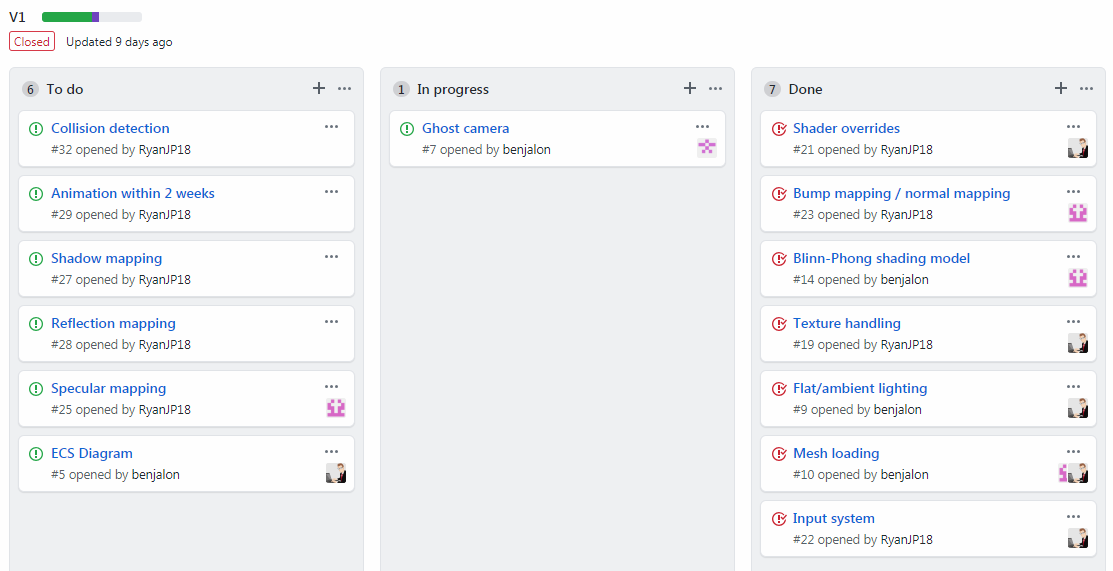
\includegraphics[width=\textwidth]{project-board.png}
\caption{An example of one of the earlier project sprints.}
\label{fig:proj-board}
\end{figure}

At the end of these sprints was an informal retrospective in which the sprint was evaluated through discussion of project progress and goals. The MoSCoW analysis was repeatedly used as a guide to re-focus priorities during these meetings to ensure that the project remained on track. 

In addition to having GitHub host the project management component of the project, Git itself was used for source control. An important decision made was to have a lock applied to the master branch to ensure that work was approved by another team member before merging. This was useful in assuring the quality of the master branch at all times, as broken code would slow down development and reduce the overall quality of the product. This also allowed pull requests to function as a type of passive white box testing, where team members were able to review all code prior to it entering the game. 

\section{Advanced Lighting}
The Blinn - Phong lighting model is an improvement upon the traditional Phong model which fixes specular reflectance calculations and combines ambient, diffuse and specular lighting into a unified framework~\cite{blinn1977models}. This model is applied on the GPU, typically at either the vertex or fragment level (Algorithm~\ref{blinnphong}). This framework provides the basis from which improvements to lighting can be built upon.

\begin{algorithm}[H]
    \begin{algorithmic}[1]
        \FORALL{fragments}
            \STATE{sample texture for color;}
            \FORALL{ambient light sources}
                \STATE{calculate ambient;}
            \ENDFOR
            \FORALL{non-ambient light sources}
                \STATE{calculate diffuse;}
                \STATE{calculate specular;}
            \ENDFOR
            \RETURN{color + ambient + diffuse + specular};
        \ENDFOR
    \end{algorithmic}
\caption{Blinn-Phong model.}\label{blinnphong}
\end{algorithm}

Bump mapping is a technique which uses an additional set of normals generated from a map texture in the lighting calculations to provide artificial detail to meshes. This is typically applied  by transforming the view position and light source into tangent space, these are then used alongside the generated normals as opposed to those from the original mesh. This process is outlined in Algorithm~\ref{bumpmapping}.

\begin{algorithm}[H]
    \begin{algorithmic}[1]
        \FORALL{fragments}
            \STATE{sample normals from map;}
            \STATE{convert view to tangent space;}
            \STATE{convert vertex to tangent space;}
            \FORALL{non-ambient light sources}
                \STATE{convert light to tangent space}
                \STATE{apply blinn-phong model}
            \ENDFOR
        \ENDFOR
    \end{algorithmic}
\caption{Application of bump mapping on shader.}\label{bumpmapping}
\end{algorithm}

By combining these techniques with a variety of novel light sources, these techniques are able to produce realistic scene lighting. A final gamma correction tweak is then applied to the colour result to remove monitor biases.

\section{Procedural Content Generation}
A major design challenge with games is how to keep the player entertained over an extended period of time. A highly popular approach to this problem is procedural content generation (PCG). PCG aims to randomise parts of the game on subsequent playthroughs and/or during different parts of the game itself. Whereas classically new content would all have to be designed and implemented, PCG seeds and generated new levels, worlds etc. from a set of rules and resources defined by the programmer.

Though the overall rules of the game are set, the project uses some effective and popular strategies within PCG to create a varied and interesting playing experience. The six levels visited in a single playthrough of the game are randomised at runtime, such that not only is each level different from one another, but they are also different every time the game is played. This variety and replayability is thus achieved without having to hard-design any individual levels.

\section{Bone Animation}
Animation has traditionally been a difficult problem to solve in graphics. 3D solutions typically involve some manipulation of vertex positions at different important points, known as key frames, in the animation time line. Between these key frames, interpolation is used to derive a smoother and more natural movement. A naive approach would then apply this vertex displacement at each frame directly to the mesh vertices, however such an approach will distort the mesh in an unnatural way. 

More effective approaches to animation instead focus on rigging the vertices to a skeletal structure and applying the displacement to the bones instead, a method used in both standard bone animation and in motion capture. The benefit of such an approach is that the displacement appears more realistic where all vertices relating to a specific bone are offset together. For each bone, the total displacement is calculated from the culmination of its transformation matrix, the displacement from vertex to bone and the weight of the attachment (Equation~\ref{equation-bones}).

\begin{equation}
    \sum_{i=0}^n M_i d_i w_i\label{equation-bones}
\end{equation}
This equation illustrates the offset calculation for bone animation. Here n is the number of bones, M is the global transform, d is the displacement and w is the weight.

\section{Particle Effects}
Particle systems are a powerful technique for recreating complicated effects such as fire or gasses. Particle systems are constructed from a pool of simple alpha-blended 2D objects, an emitter and an update mechanic.

Particles are created at the source emitter from a fixed template with some randomness injected into their positions, velocities and appearance. Upon creation they are designated a lifespan to prevent them deviating too much from their source. When this expires, they are added to the pool ready for re-creation. Algorithm~\ref{particle-update} illustrates how particles could be updated within a particle system.

\begin{algorithm}[H]
    \begin{algorithmic}[1]
        \WHILE{$deadParticles > 0$}
            \STATE{respawnParticle;}
        \ENDWHILE
        \FORALL{particles}
            \STATE{particle.life -= delta;}
            \IF{$particle.life > 0$}
                \STATE{particle.position -= particle.velocity * delta;}
                \STATE{particle.colour.alpha -= delta;}
            \ELSE
        		\STATE{deadParticles++;}
            \ENDIF
        \ENDFOR
    \end{algorithmic}
\caption{Particle update system.}\label{particle-update}
\end{algorithm}

\chapter{Implementation}
When the game starts, the player is transported to the main hub, a room which connects them to the procedural dungeon through a portal (Figure \ref{fig:startRoom}). At the back of the room is the exit door which opens when the six keys are gathered to complete the game (Figure \ref{fig:door}). The scene itself is lit with a variety of different light sources and particle effects (Figure \ref{fig:key} shows a key). The dungeon is populated by enemies who will attack the player if they are in range. Both the player and the enemies can shoot fireballs (Figure \ref{fig:fireball}) to damage their opponent.

\begin{figure}[H]
\centering
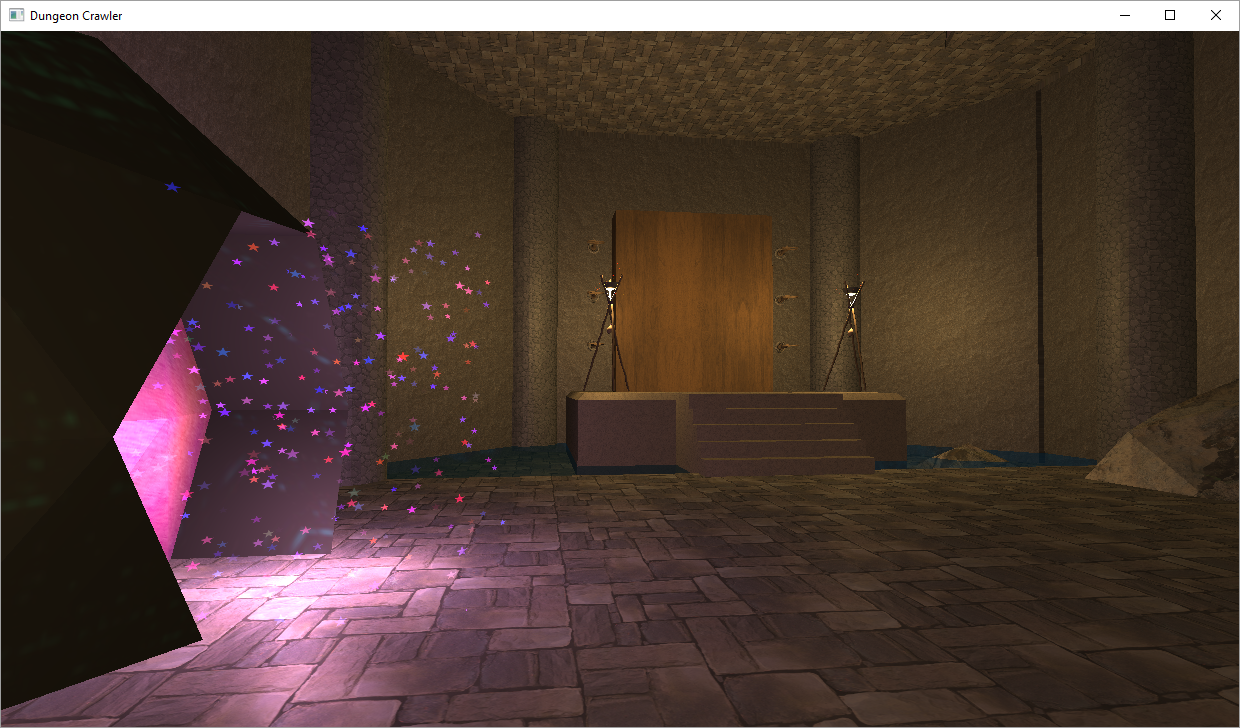
\includegraphics[width=0.8\textwidth]{startRoom.PNG}
\caption{The starting area for the player.}
\label{fig:startRoom}
\end{figure}
\begin{figure}[H]
\centering
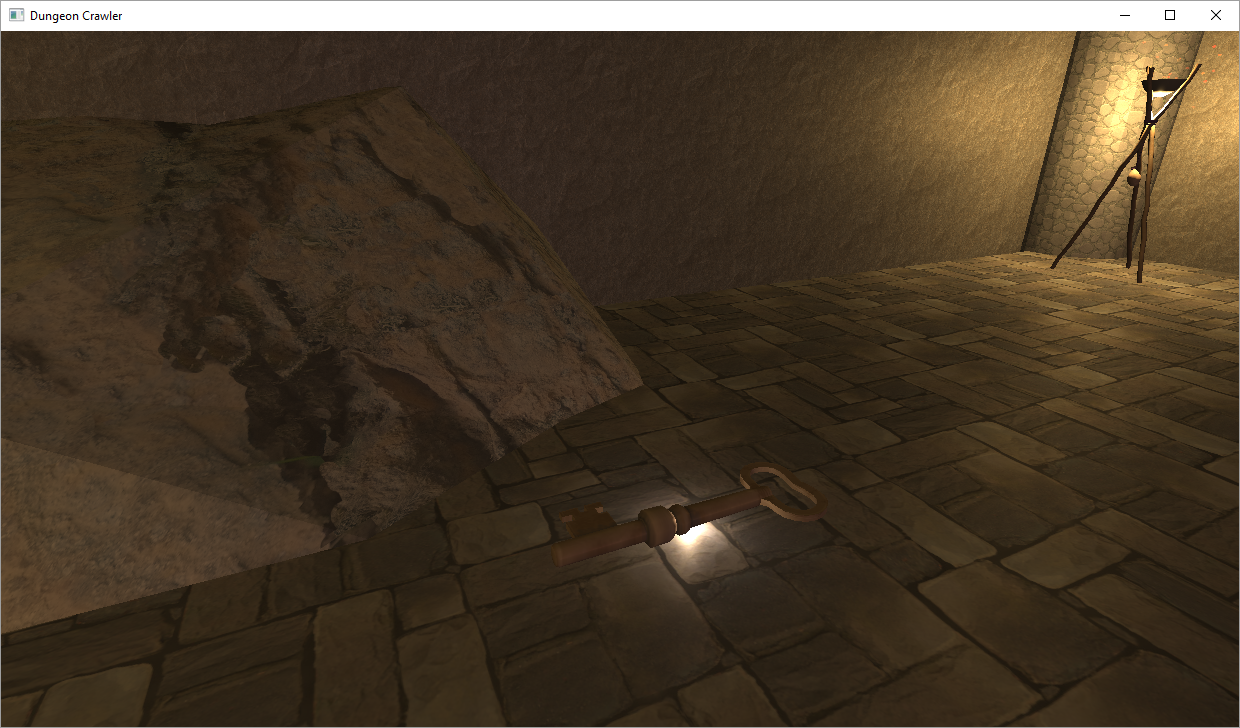
\includegraphics[width=0.8\textwidth]{keyandlight.PNG}
\caption{A key that unlocks the final door in the game.}
\label{fig:key}
\end{figure}
\begin{figure}[H]
\centering
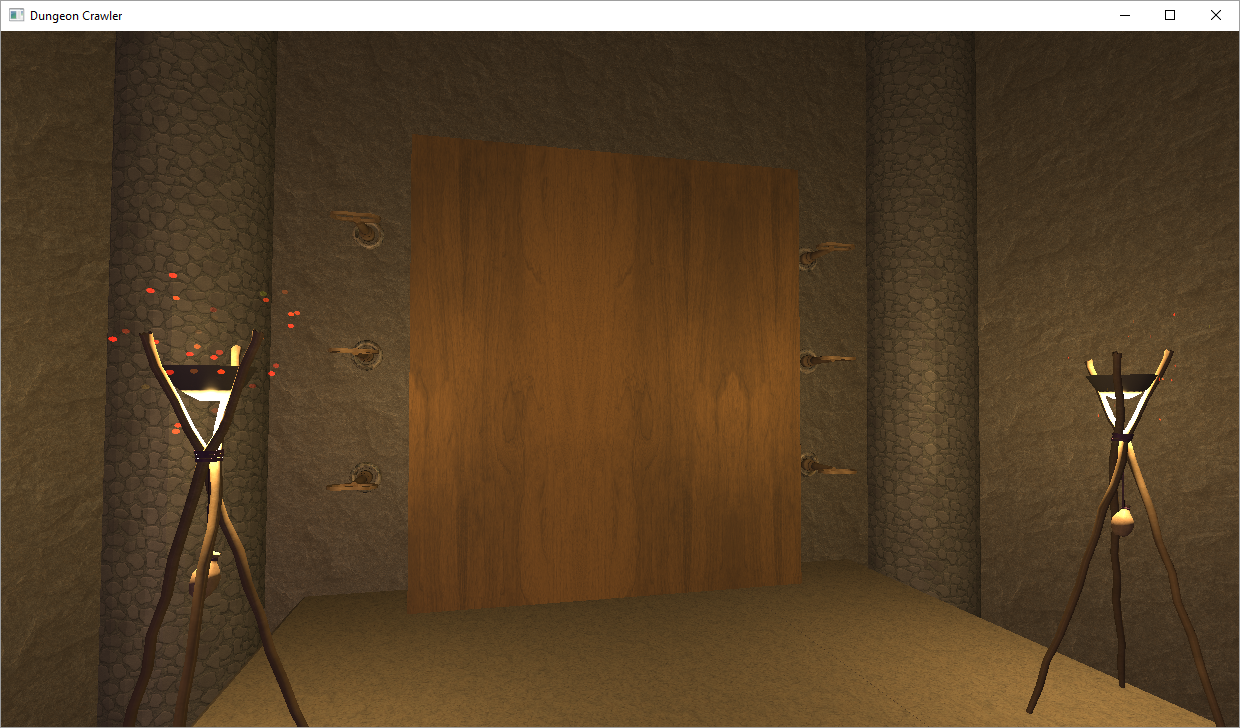
\includegraphics[width=0.8\textwidth]{doorWithKeys.PNG}
\caption{The final door with all six keys in place.}
\label{fig:door}
\end{figure}
\begin{figure}[H]
\centering
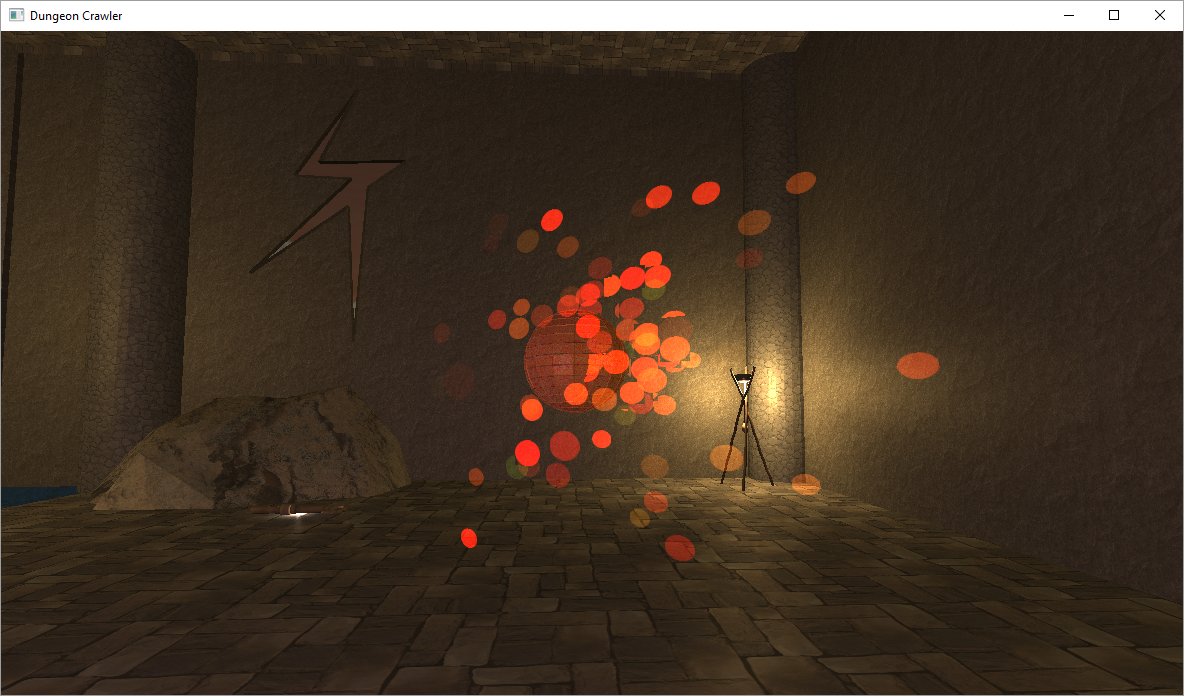
\includegraphics[width=0.8\textwidth]{fireball.PNG}
\caption{Character shooting  a fireball.}
\label{fig:fireball}
\end{figure}

\section{Game Engine and Architecture}\label{section-ecs-imp}
The ECS pattern was implemented using the \emph{EnTT} library, an extremely efficient implementation of component pools and system iterators. This library only provided low-level tools and still needed to be fashioned into an extendable engine. The primary challenge here was abstraction, allowing team members to program game logic in an elegant environment.

The structure of the engine can be divided into two parts. The low level of the engine uses only very simple object-oriented design to define the underlying game application and ECS system (figure~\ref{fig:uml}); most of the heavy lifting of the ECS implementation is done through template metaprogramming and static polymorphism as opposed to OOP. The high level uses the ECS architecture to script the game.

\begin{figure}[H]
    \centering
    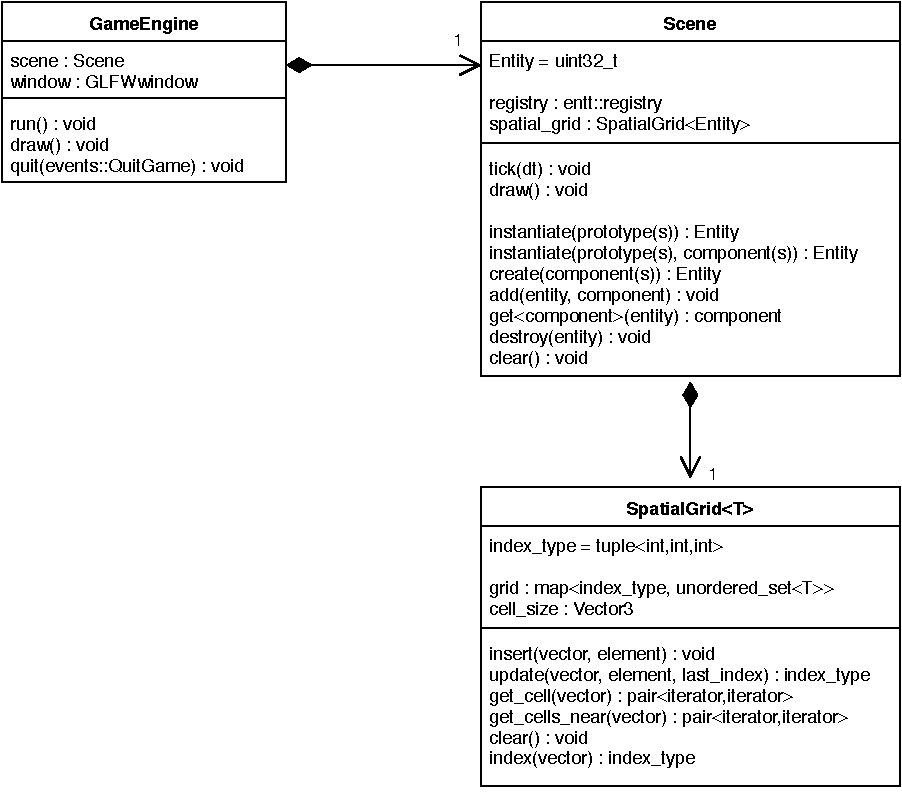
\includegraphics{UML.pdf}
    \caption{Simplified UML diagram showing the straightforward object-orientation of the lowest level of the engine}
    \label{fig:uml}
\end{figure}

The \texttt{Scene} class contains the registry of entities and components. It provides a number of methods for instantiating, accessing and manipulating entities and components as intuitively as possible, with the help of template fold expressions and initialiser lists.

Components are easily defined as simple data structs (\texttt{Components.h}). In order to ease the instantiation of entities, namely to remove the need to define all of their components every time, \emph{prototypes} are implemented to allow the definition of different types of entities and which components they are expected to possess. A system is defined as a lambda registered for use with a particular set of components.

Metaprogramming is used to ease these definitions for users. Macros are provided which automatically register the definitions in the correct collections through the curiously recurring template pattern (CRTP). For example, the collections of systems then simply becomes a vector of (wrapped) lambdas which are all invoked each game tick. This is implemented for systems and prototypes in \texttt{Systems.h} and \texttt{Prototypes.h}, with custom definitions placed in \texttt{Systems.cpp} and \texttt{Prototypes.cpp}.

Events are provided in a similar fashion. An \emph{event} is a simple data struct containing information of a specific event which can be invoked anywhere from system logic (\texttt{Events.h}). A \emph{response} is again a function defined using a macro which triggers when its corresponding event occurs (\texttt{Events.cpp}). Events can be invoked either instantaneously (e.g. for system key presses) or enqueued for the end of the game tick (e.g. for collision responses).

The \texttt{GameEngine} object controls the main game loop, implemented as a \texttt{while} loop on the \texttt{glfwWindowShouldClose} flag. The game loop is split into two key sections: ticking and drawing. Ticking is the computation of all game logic, whilst drawing is the rendering of all entities to the screen. Fundamentally, these two functions are decoupled in order to prevent lag in expensive rendering from affecting the game logic itself.

\texttt{GameEngine} possesses a constant \texttt{GAME\_RATE}, which is set to 60 Hz. This is the target number of times, per second, the game logic is ticked. GLFW's native timer is used to perform this, as well as provide delta time to the game logic (i.e. each system). Drawing is then performed after ticking, but only if we are running up to the target speed -- if it is already time for the next update after ticking but before drawing, the drawing is skipped. This gives the frame rate the flexibility to drop in order to allow the game logic to maintain speed, rather than restricting the logic performance by the rendering performance.

A notable direct member of the \texttt{Scene} is a \texttt{SpatialGrid}. This is an implementation of regular space partitioning to improve the efficiency of the collision system. The central concept is that a rough check for proximity can rapidly filter out the entities one may definitely not be colliding with, and thus reduce the number of precise collision checks each tick.

The grid consists of an (ordered) map of indices to (unordered) sets of entities. An index is a 3-tuple of integers, a 3D grid spanning indefinitely in positive and negative directions. A \texttt{SpatialGridSystem} updates each collidable entity's location in the grid before the \texttt{CollisionSystem} queries them, obtaining a set of nearby entities to perform precise collision checks with.

As performance is key in this situation, the \texttt{SpatialGrid} has carefully-selected containers, efficiently uses iterators and static function variables for operations such as the union, and makes \texttt{TransformComponent}s remember their previous index for fast updating.

\section{Artificial Intelligence}
A finite state machine is used to manage the enemy behaviour and provide simple artificial intelligence to enemies in the game (Figure \ref{fig:fsm}).
\begin{figure}[ht]
\centering
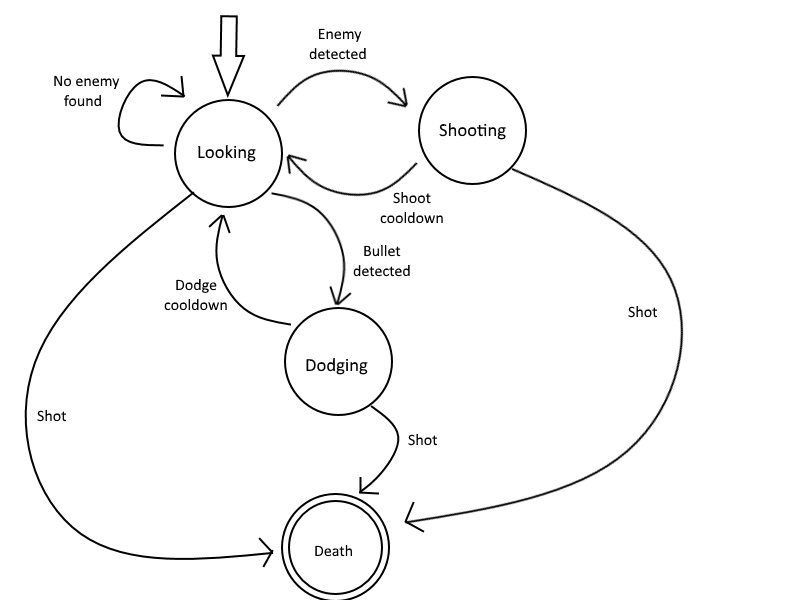
\includegraphics[width=0.8\textwidth]{fsm.png}
\caption{Finite State Machine used for enemy artificial intelligence.}
\label{fig:fsm}
\end{figure}
These enemies move between three active states and one final death state. The default state, ``looking'' has the enemy search its detection range for either the player or a fireball. If it finds a player it then shoots a fireball at the player, beginning their fireball cooldown. If the enemy detects that they are being fired at by the player, they attempt to dodge it, beginning a dodge cooldown. If at any point the enemy is intersected by a fireball projectile, it dies and is removed from the world.       
The enemy rotates to follow the player when it detects that they have entered its detection radius. This rotation is determined by taking a point between them and calculating an orientation using the dot product between the two (Equation~\ref{rotation}). The enemy then is able to fire at the player by using the determined angle.

\begin{equation}
    \cos \theta =\frac{u . v}{||u|| ||v||}\label{rotation}
\end{equation}
\begin{equation}
    \theta = \arccos \Big(\frac{ u . v }{ ||u|| ||v||}\Big)
\end{equation}

\section{Procedural Content Generation}
When a new level is visited in the game, it must be randomly generated at and only at that time. A number of key specifications immediately arise:

\begin{itemize}
    \item The PCG must be fast and efficient so as not to disturb play.
    \item The PCG must incorporate a sufficient randomness factor to maintain variety.
    \item In conflict with above, the PCG must remain within the bounds of creating an effective and interesting level.
    \item The PCG must be as parameterisable as possible to allow fine-tuning of the end result.
\end{itemize}

PCG can take drastically different forms depending on the style of game and levels desired. As it is used to generate dungeon interiors, the approach implemented follows this overall algorithm:

\begin{enumerate}
    \item Fill a desired area with a perfect maze using depth-first `search'.
    \item Increase the sparsity of the maze by retracting dead ends.
    \item Place a number of rooms of random sizes at random locations, in space not yet used.
    \item Connect each room to the overall maze.
    \item Finally, convert this generated grid into an actual scene with models.
\end{enumerate}

The depth-first `search' uses a stack and backtracking to fill the entire area with a perfect maze. A perfect maze means that there are no loops -- the entire path forms a tree. This entire area is naturally (for now) connected, so is assigned the first area ID of 1.

As-is, this perfect maze is too dense. A simple way of increasing the sparsity is to find every dead end and retract them iteratively by filling them back in, by some desired amount.

After sparsification, there is a considerable amount of solid space around the maze corridors. A desired number of rooms are placed randomly in this free space. The sizes of these rooms are randomly sampled from a desired range -- if not all the rooms could be placed successfully, this is repeated with the maximum size reduced until completion. As each of these rooms are disconnected, they are assigned increasing area IDs.

The final step is to connect each room to the overall maze, and thus to each other. From each room, a path randomly sprawls out: if it opens up to the already-connected areas (tracked through a cache of IDs) then it terminates. Otherwise, is randomly selects a direction that would lead to a dead end and continues until success.

This sprawling path is prevented from turning back on itself by avoiding its own area ID. This still leaves a chance that it can become stuck behind itself in a corner of the grid with nowhere else to go. Should this happen, the path is deleted and the algorithm merely tries again until success. Therefore, it is a Las Vegas algorithm: through the use of randomness, it will always result in a valid solution after \emph{some} amount of time. Due to the small size of the problem space, this expected runtime is far too low to impact the player.

Converting this grid into a playable scene is a matter of spawning wall models for each cell. Only five models are needed to define the entire layout, with each piece rotated as necessary to correctly represent the corners, junctions etc. of the dungeon.

\chapter{Testing}
Unlike more rigid development patterns, the Agile methodology expects that testing is a continuous process through each iterative development cycle. For this reason, the project management integrated passive white-box testing through a locked master branch with enforced pull requests. For any code to be merged into the master branch, it had to pass a sanity check by being approved by another member of the team.

In addition to this passive testing, a more definitive phase of testing was undertaken at the end of the final sprint in the form of black-box testing (Figure~\ref{test-sprint}). Here, all bugs were labelled with a priority depending on their influence on the final product. In particular, must fix refers to game-breaking bugs and should fix are those which actively detract from the overall experience.

\begin{figure}[ht]
\centering
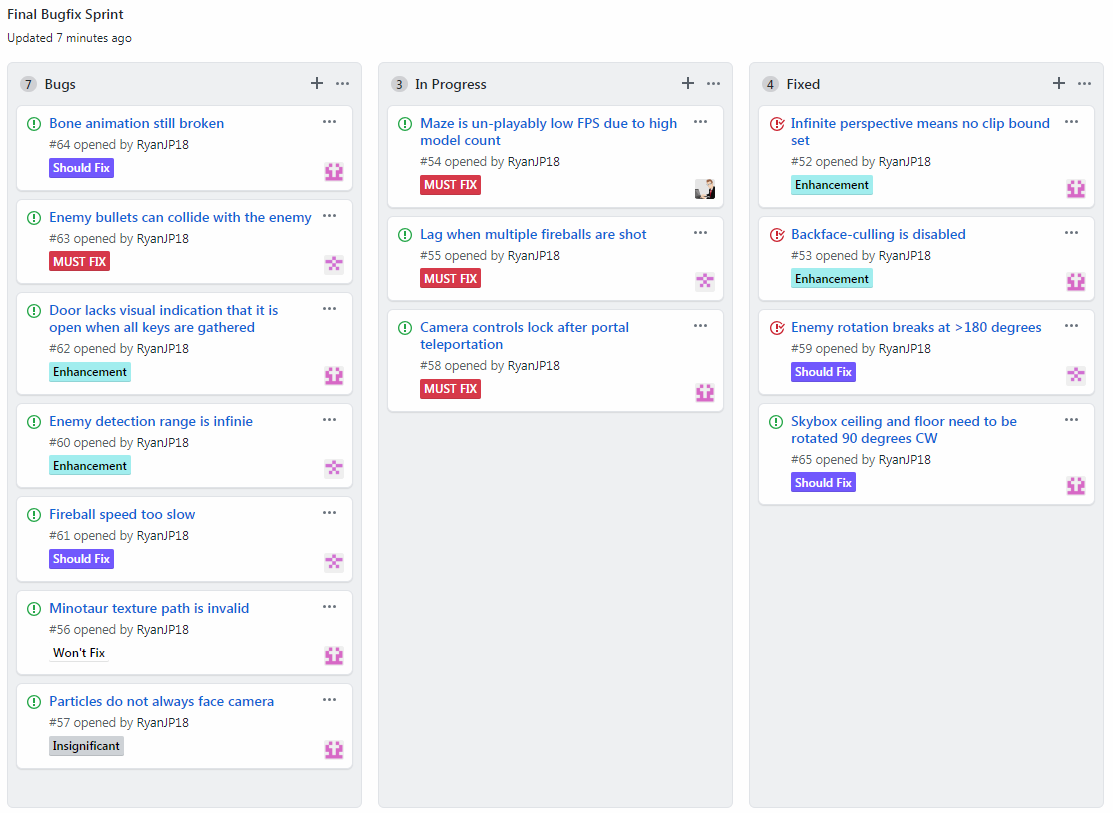
\includegraphics[width=\textwidth]{test-sprint.png}
\caption{The final test sprint during the bug fixing period.}
\label{test-sprint}
\end{figure}
Finally, requirements testing was carried out to assure the basic functionality of the product (Figure~\ref{requirements-test}).

\begin{figure}[H]
	\centering
	\begin{tabular}{p{0.25\textwidth}||c||p{0.55\textwidth}}
		Requirement & Result & Testing Notes \\ 
		\hline 
		\hline 
		The game must have a clear and objective ending & Pass & Collecting the six keys from the procedural dungeon causes the main door to unlock, allowing the player to complete the game \\ \hline
		The game must be verified completeable with no game-breaking bugs & Pass &  There were a number of game-breaking bugs present in earlier versions of the game but these were corrected in the final bug-fixing sprint \\ \hline
		The current game state must be clear & Acceptable & This could be made clearer, though the current UI is sufficient \\ \hline
		The game must have an enemy threat & Pass & The minotaur enemies target the player upon detection and fire back at them \\ \hline
        The framerate must remain stable & Acceptable & The frame-rate is reasonably stable, though it struggles when a large number of meshes are present on the screen at one time \\ \hline
        The scene must be believable as a fantasy dungeon & Pass & The scene was designed with this objective in mind, furthermore assets such as torches and the minotaur enemies were chosen specifically to not clash with this idea \\ \hline
        The scene lighting must be appear realistic & Pass & Techniques such as the Blinn - Phong lighting model and gamma correction are applied to meet this aim \\ \hline
         The player must collide with walls, projectiles and game objects & Acceptable &  The collision radius on several objects could be improved, most notably on keys and fireballs \\ \hline
	\end{tabular}
	\caption{Requirements testing. \label{requirements-test}}
\end{figure}

\chapter{Conclusion}
The iterative development process was something which proved effective at all points in the project. By tasking each member with work items, it helped ensure that development was transparent and flexible. This was particularly useful during phases of rapid development and led to relatively little crowding in the code base. However, as with any project there were various challenges in development. These issues mainly centred around the use of unfamiliar technologies such as ECS and animation which caused development to stall at times. To some extent, it could be argued that these issues were unavoidable as a learning experience required by the team. However, the learning curve could likely have been managed better through shorter sprint duration to ensure regular checkup on progress and assistance from other team members.

%Put in perspective of the moscow
In considering the initial project MoSCoW analysis (Figure~\ref{moscow-1}), the ``must have'' and ``should have'' objectives were all thoroughly completed. Several ``could have'' tasks were chosen to be completed, particularly particle effects and multiple environments to provide the game with some additional detail. Others such as UI and water were attempted, though left slightly incomplete due to time constraints. The resulting game appears coherent from a graphical perspective, though the gameplay could be argued to be a weakness due to its simplicity.

%Conclude achievements
As a project, it could be argued that DunCraw: The Third Realm has been successful. A 3D game has been produced with a number of advanced features. Testing also shows that the design goals of the project were met (Section~\ref{requirements-test}), which coupled with the completion of the primary MoSCoW objectives indicate a degree of project consistency.  

%Discuss feature development if you had more time
That being said, there is still much that could be improved on the project. The biggest weakness is arguably in its lack of variation of content. The PCG and enemy AI provide a framework to rapidly increase gameplay depth and variety, but in their current state are perhaps over-engineered for their relative impact on the game. Were the project to be repeated again, more emphasis would be placed on implementing these systems earlier in development to allow them greater influence on the content. Likely the biggest strength of the project is in the overall quality of its engine architecture and moving forward, it would be simple to capitalise on this.

\bibliographystyle{unsrt}
\bibliography{references}

\chapter*{Contributions}
The team has agreed on a 33\% contribution each as each member completed allocated tasks and attended meetings. Not listed are tasks completed as a team such as planning and report writing.

\begin{figure}[H]
	\centering
	\begin{tabular}{c|p{0.8\textwidth}}
		Member & Contributions \\ 
		\hline 
		\hline 
		Ben Longhurst & \begin{itemize}
			\itemsep0em
			\item First person camera
			\item Enemy AI and state management
			\item Shooting mechanic
			\item Project management
			\item Death condition
            \item Sound effects
		\end{itemize} \\ \hline
		Ryan Phelan & \begin{itemize}
			\itemsep0em
			\item Scene lighting
			\item Advanced shaders (skybox, water, bump mapping etc.)
			\item Creating scene assets
			\item Model loader and buffer setup
			\item Bone animation
			\item Keys and win condition
			\item Particle system
			\item UI overlays
		\end{itemize} \\ \hline
		Sam Griffiths & \begin{itemize}
			\itemsep0em		
			\item Engine design and code architecture
			\item ECS system
			\item Event messaging system
			\item Collision system and spatial grid
			\item Procedural content generation
			\item Code optimisation
		\end{itemize} \\
	\end{tabular}
	\caption{Team contribution breakdown.}
\end{figure}

\end{document}